\Chapter {Tesztelés a gyakorlatban}
Minden teszt esethez tartoznak különböző információk, amik változnak a cég által használt rendszertől függően. Lehetséges, hogy egy teszt esetet létre tud hozni a kreálója, minden mellék információ megadása nélkül, de általában van néhány alap feltétel is amiket az én programom keretében \aref{table:template}-es táblázat mutatja be.\\

\label {table:template}
\label {table:testcase}
\label {table:successcase}
\label {table:addnode}
\label {table:jtree}
\label {table:ekvivalencia}
\label {table:kombináció}

\label {tab:console}
\label {tab:modify}
\label {tab:program}
\label {tab:tree}
\label {tab:login}

\begin{table} [h]
	\begin{center}
		\begin{tabular}{ | p{6cm} | p{6cm}| } 
			\hline
			A teszt készítője & Orosz Dénes Milán  \\ 
			\hline
			A teszt fajtája & Sikeres bejelentkezési teszt  \\ 
			\hline
			A teszt elő követelményei & A program bármely futtatható verziója  \\ 
			\hline
			A teszt stratégia verziószáma & 1.0 \\
			\hline
			Kapcsolat(ha van) & Sikertelen login teszt \\
			\hline
		\end{tabular}
	\label{tab:template}
	\caption{A teszt esethez tartozó információk.}
	\end{center}

\end{table}
Minden teszt eset 3 vagy 4 oszlopból áll. Az első oszlopban a lépés sorszáma, a másodikban  maga a lépés van megfogalmazva, a harmadik és negyedik oszlop pedig az elvárt eredményt, illetve a lépéshez tartozó bemenetet tartalmazzák, viszont előfordulhat, hogy a bemeneteket egy másik táblázatban tárolják. Példát erre  \aref{table:testcase}-es táblázat mutat.\\

\begin{table}[h]
\begin{center}
	\resizebox{\textwidth}{!} {
\begin{tabular}{ |p{3cm}|p{5cm}|p{5cm}|p{5cm}|} 
	\hline
	 Lépés sorszáma & A tesztlépés leírása & A tesztlépéshez tartozó bemeneti érték (ha van) & A tesztlépés elvárt értéke  \\ 
	\hline
	1. & & &  \\ 
	\hline
	2. & & &  \\ 
	\hline
	3. & & & \\
	\hline
	4. & & & \\
	\hline
\end{tabular}
}
\end{center}
	\caption{Egy teszt eset teszt lépések nélkül}
	\label{table:testcase}
\end{table}

\Aref{table:successcase}-mas táblázaton látható, az én programomhoz tartozó bejelentkezést tesztelő teszt esetnek a lépéssorozata és a hozzá tartozó bemenetek, illetve az elvárt eredmények.

\begin{table} [h]
	\begin{center}
		\resizebox{\textwidth}{!} {
			\begin{tabular}{ |p{3cm}|p{5cm}|p{5cm}|p{5cm}| } 
				\hline
				Lépés sorszáma & A tesztlépés leírása & A tesztlépéshez tartozó bemeneti érték (ha van) & A tesztlépés elvárt értéke  \\ 
				\hline
				1. & Indítsd el a programot. & - & A program elindul és egy bejelentkező ablak látható a képernyő közepén.  \\ 
				\hline
				2. & Írd be a megadott teszt adatokat. & Felhasználó név: test \newline Jelszó: test123 & A felhasználónév olvasható, viszont a jelszó helyén **** látunk.\\ 
				\hline
				3. & Kattints rá a "login" gombra. & - & A gomb megnyomása után sikeresen bejelentkezünk. \\
				\hline
				4. & Lépj ki a programból az x segítségével. & - & A program bezáródik. \\
				\hline
			\end{tabular}
		}
	\end{center}
	\caption{A programhoz tartozó sikeres bejelentkezés teszt esete}
	\label{table:successcase}
\end{table}

\Aref{table:addnode}-es táblázatban látható a program egyik fő funkciójának a tesztje, amivel a fa struktúrához lehet hozzáadni egy fő elemet, illetve ha szeretné a felhasználó akkor még plusz levél elemeket a fő elem alá, viszont a teszt ezt a részt már nem tartalmazza, mivel egy másik funkcionális teszt tartalmazza azt.

\begin{table} [h]
	\begin{center}
		\resizebox{\textwidth}{!} {
			\begin{tabular}{ |p{3cm}|p{5cm}|p{5cm}|p{5cm}| } 
				\hline
				Lépés sorszáma & A tesztlépés leírása & A tesztlépéshez tartozó bemeneti érték (ha van) & A tesztlépés elvárt értéke  \\ 
				\hline
				1. & Indítsd el a programot és jelentkezz be. & Felhasználó név: test \newline Jelszó: test123 & A program elindul és a bejelentkezés is sikeres.  \\ 
				\hline
				2. & Kattints a "New Node" gombra. & - & 3 új gomb jelenik meg ("Get Information","Add Node(s)", "Back"), illetve egy szöveget elfogadó rész, ami az új elem nevét várja értékként.\\ 
				\hline
				3. & Írd be a teszt adatot, majd kattints a "Get Information" gombra és utána az "Add Node(s)" gombra & Teszt adat: "érték" & A gombok megnyomása után a fa struktúrában létrejön az "érték" nevű levél és kijelölésre kerül. \\
				\hline
				4. & Lépj ki a programból az x segítségével. & - & A program bezáródik. \\
				\hline
			\end{tabular}
		}
	\end{center}
	\caption{A fa struktúra módosítása új elem hozzáadásával}
	\label{table:addnode}
\end{table}

\newpage

\Aref{table:jtree}-ös táblázatban látható a program egy másik fő funkciójára írt teszt eset. A fában lévő elemek reprezentálják a programhoz csatolt adatbázis táblaneveit és ezen táblák adatait lehet kiíratni egy kattintással. Ha duplán kattintunk, akkor is csak egyszer íródnak ki az elemek, viszont lenyílásra kerül a fában a tábla és ha a most már látható levelekre kattintunk, akkor a csak hozzá tartozó elemek kerülnek kiírásra.

\begin{table} [h]
	\begin{center}
		\resizebox{\textwidth}{!} {
			\begin{tabular}{ |p{3cm}|p{5cm}|p{5cm}|p{5cm}| } 
				\hline
				Lépés sorszáma & A tesztlépés leírása & A tesztlépéshez tartozó bemeneti érték (ha van) & A tesztlépés elvárt értéke  \\ 
				\hline
				1. & Indítsd el a programot és jelentkezz be. & Felhasználó név: test \newline Jelszó: test123 & A program elindul és a bejelentkezés is sikeres.  \\ 
				\hline
				2. & Kattints a fa struktúrában egy fő elemre. & - & Az adatok amiket tartalmaz az elem kiírásra kerülnek a program alsó részén.\\ 
				\hline
				3. & Dupla kattintással nyisd le ugyanezt az elemet és kattints rá az egyik alatta lévő levélre & - & Az előzőleg kiírt adatokból, most csak a levélhez tartozó rész íratódik ki a program alsó részén. \\
				\hline
				4. & Lépj ki a programból az x segítségével. & - & A program bezáródik. \\
				\hline
			\end{tabular}
		}
	\end{center}
	\caption{A fa struktúrából adat kinyerés}
	\label{table:jtree}
\end{table}

\Section{Fekete doboz tesztelési módszerek a gyakorlatban}
\subsection{Ekvivalencia particionálás} \Aref{table:ekvivalencia}-es táblázatban láthatunk egy példát az ekvivalencia particionálásra. Ez a példa a programom bejelentkező felületére hoz egy példát.

\begin{table} [h]
	\begin{center}
		\begin{tabular}{ | p{4cm} | p{4cm}|  p{4cm} |} 
			\hline
			Bemenet & Érvényes & Érvénytelen  \\ 
			\hline
			Felhasználónév & V1: test \newline V2: admin & I1: üres \newline I2: bármi más szó  \\ 
			\hline
			Jelszó & V3: test123 \newline V4: admin & I3: üres \newline I4: bármi más szó  \\ 
			\hline
		\end{tabular}
	\end{center}
	\label{table:ekvivalencia}
	\caption{Példa az érvényes és érvénytelen adatokra}
\end{table}
\newpage
Az alábbi táblázatban látható néhány lehetséges kombináció a bejelentkezéshez. Minden sorhoz tartozik egy felhasználó név és egy jelszó, illetve az adott kimenetel. Fontos, hogy ha egy olyan felhasználót vagy jelszót adunk meg, ami érvénytelen, ahhoz már másik érvénytelen adat ne kerüljön, ugyanis ott nem tisztázható, hogy melyik okozza a hibás működést.

\begin{table} [h]
	\begin{center}
		\begin{tabular}{| p{3cm} | p{3cm} | p{3cm} | p{3cm} |}
			\hline
			Teszt & Felhasználónév & Jelszó & Kimenet \\
			\hline
			T1 & V1 & V3 & Érvényes \\
			\hline
			T2 & V1 & V4 & Érvényes \\
			\hline
			T3 & V2 & V3 & Érvényes \\
			\hline
			T4 & V2 & V4 & Érvényes \\
			\hline
			T5 & V1 & I3 & Érvénytelen \\
			\hline
			T6 & I1 & V3 & Érvénytelen \\
			\hline
			... & & & \\
			\hline
			\end{tabular}
	\end{center}
	\caption{Példa az ekvivalencia particionálási táblázatra}
\end{table}

\subsection{Határérték-elemzés} A programon belül a határérték elemzést bármelyik részre lehet alkalmazni, ahol numerikus megfelelés alapján történik a vizsgálat. Fontos tudni, hogy akkor is használható, ha a megfeleltetésünk nem két határ érték közé tartozik, hanem mondjuk az összes pozitív szám jó a feltétel szerint. Tipikusan hibás operátorok, vagy ciklus be és kilépési pontoknál lévő hibákat találunk meg ezzel a módszerrel. Példát a következő lista tartalmaz.

\begin{itemize}
	\item Határértékek a leadott SQL parancsok esetén
	\item Select
		\begin{itemize}
			\item Megfelelő számok 0 - +$\infty$
			\item Tesztelendő számok: -999, -2, -1, 0, 1, 2, 999 
		\end{itemize}
	\item Update
		\begin{itemize}
			\item Megfelelő számok 1 - +$\infty$
			\item Tesztelendő számok: -999, -1, 0, 1, 2, 999 
		\end{itemize}
	\item Delete
		\begin{itemize}
			\item Megfelelő számok 1 - +$\infty$
			\item Tesztelendő számok: -999, -1, 0, 1, 2, 999 
		\end{itemize}
	\item Alter
		\begin{itemize}
			\item Megfelelő számok 0
			\item Tesztelendő számok: -1, 0, 1
		\end{itemize}
	\item Insert
		\begin{itemize}
			\item Megfelelő számok 1 - +$\infty$
			\item Tesztelendő számok: -999, -1, 0, 1, 2, 999 
		\end{itemize}
	\item Create
		\begin{itemize}
			\item Megfelelő számok 0
			\item Tesztelendő számok: -1, 0, 1
		\end{itemize}
	\item Drop
		\begin{itemize}
			\item Megfelelő számok 0
			\item Tesztelendő számok: -1, 0, 1
	\end{itemize}
\end{itemize}
\newpage
\subsection{Döntési tábla tesztelés} A programon belül a döntési tábla tesztelést általában egy jól körülírható funkcióra szokták alkalmazni, mint sem hogy a teljes alkalmazásra. Tételezzük fel, hogy a program a lefuttatott sql kód alapján meg akar keresni egy személyt, a táblák között és ehhez 3 paramétert vár el a kódban.\\
\begin{itemize}
	\item Név
	\item Beosztás
	\item Kód 
\end{itemize}

Ezeknek a paramétereknek 2-2 lehetséges bemenetük van. Vagy helyes a megadott adat, vagy helytelen. Az egyszerűség kedvéért, nem foglalkozunk azzal, hogy üres bemenetet adunk meg.\\

Létezik egy negyedik sor a táblához ami a kimenetet fogja nekünk adni. Ebben a szituációban ezek hibaüzenetek lesznek, mert valamelyik adat nem felel meg a kritériumoknak. A tábla a következőképpen néz ki.

\begin{figure} [h]
	\begin{center}
		\begin{tabular}{| p{2cm} | p{2cm} | p{2cm} | p{5cm} |}
			\hline
			Név & Beosztás & Kód & Hibaüzenet\\
			\hline
			& & & Helyes adat megadás\\
			\hline
			+ & & & Nem található a név\\
			\hline
			& + & & Nem található a beosztás\\
			\hline
			&  & + & Nem található a kód\\
			\hline
			+ & + & & Nem található a név és a beosztás\\
			\hline
			+ & & + & Nem található a név és a kód\\
			\hline
			& + &  +& Nem található a beosztás és a kód\\
			\hline
			+ & + & + & Nem található a név, a beosztás és a kód\\
			\hline
		\end{tabular}
	\end{center}
\end{figure}

Ahol "+" jel látható, az mutatja, hogy az az adat megadásra került, viszont valamilyen hibával és így nem felel meg a kritériumnak. Minden sor 1 teszt esetet fed le, ami jelen pillanatban 8, mivel 3 bemenetünk van 2-2 fajta bemenettel és ezért a sorok száma 2*2*2 = 8 lesz.

\subsection{Állapotátmenet tesztelés} Ahogy a név is sugallja, a program állapotának változása alapján nézzük, hogy minek kellene történnie és mi az, ami valójában történik. Erre nagyon egyszerű példa tud lenni egy ATM rendszer működése, viszont a programom login rendszere is megfelel a bemutatásra. \\

A rendszerbe bejelentkezéskor meg kell adni egy felhasználó nevet és egy jelszót. Ha a helyes jelszó és felhasználó név kombináció kerül megadásra, akkor a program beenged minket, egyéb esetben, újra kell próbálkoznunk. A maximális próbálkozások száma változhat és nem is lényeges abból a szempontból, hogy hány esélyünk van a próbálkozásoknál, hanem inkább a lényeges része az állapotok és az ott lezajló események.

A jelenlegi példában 3 sikertelen próbálkozás után automatikusan bezáródik a bejelentkezési felület és a program vele együtt. A következőképpen néz ki a példa táblázat formájában.

\begin{figure} [h]
	\begin{center}
		\begin{tabular}{| p{4cm} | p{3cm} |p{3cm} |  p{3cm} |}
			\hline
			Állapot & Helyes felhasználó név & Helyes jelszó & Helytelen adat\\
			\hline
			1. próba & test\newline admin & test123 \newline admin & jelszó: test\\
			\hline
			2. próba & test\newline admin & test123 \newline admin & jelszó: test1234\\
			\hline
			3. próba & test\newline admin & test123 \newline admin & jelszó: admin123\\
			\hline
			\multicolumn{4}{|c|}{A program bezárul}\\
			\hline
			\multicolumn{4}{|c|}{A program újraindul}\\
			\hline
			1. próba & test\newline admin & test123 \newline admin & - \\
			\hline
			\multicolumn{4}{|c|}{Sikeres bejelentkezés}\\
			\hline
		\end{tabular}
	\end{center}
\end{figure}

Ilyenkor az állapotok között lehet változás. Általában a megadott helytelen adatra specializált visszajelzést kap a felhasználó. Példaként a következő táblázat szolgál.
\begin{center}	
\begin{tabular}{| p{6cm} | p{8cm} |}
	\hline
	Hiba indoka & Hibaüzenet\\
	\hline
	Helytelen felhasználó név & A felhasználó név nem megfelelő \\
	\hline
	Helytelen jelszó & A jelszó nem megfelelő\\
	\hline
	Helytelen felhasználó és jelszó & A megadott adatok nem megfelelőek\\
	\hline
\end{tabular}
\end{center}

\subsection{Használati eset tesztelés} Talán a legösszetettebb teszt esetek a használati eset tesztelésnél jönnek létre. Általában több egység kombinált működését teszteljük, ami elég hosszadalmas eseteket tudnak létrehozni. \\

Ha az alkalmazásnak van 1 fő funkciója, ami mellé tartalmaz még néhány más, de kevésbé fontos részt a működés szempontjából, akkor 1 fő ágat hozunk létre, ami a fő funkciót teszteli, majd ezután térünk rá a mellék ágakra. \\

Mostanában azért elég ritka az ilyen fajta alkalmazás, inkább több szétterjedő ágról beszélhetünk. Ilyenkor több teljes ágakat tesztelő részt készítünk, és utána nézzük meg a kevésbé fontos funkciókat.

Fontos tudni, hogy ilyenkor a megrendelő által megadott feltételeket teszteljük, ami elképzelhető, hogy csak a következő lesz: "Hozhassak létre egy új táblát az adatbázisban adatokkal, majd a fa struktúrában ezt el tudjam érni." \\

Ilyenkor ez az ő szemében csak néhány kattintás, viszont tesztelési szempontból egy nagyon sok funkciónak az összetett munkáját jelenti és ezért úgy kell megírni a teszt esetet is, hogy minden használt funkciónál ellenőrzésre kerüljön először a fő rész, és utána a mellék ágak is.\\

Ugyanennél a példánál maradva a következőképpen néznek ki a funkciók:
\begin{itemize}
	\item Bejelentkezés
	\item SQL kód megírása / bemásolása
	\item A tábla feltöltése adatokkal
	\item A fához az új tábla hozzáadása (beleértve a leveleket is)
	\item A fában lévő új elem ellenőrzése
\end{itemize}

Miután ez a fő folyamat lefutott és hiba nélkül működik a következő lépések jönnek:

\begin{itemize}
	\item A bejelentkezés ellenőrzése
		\begin{itemize}
			\item felhasználónév és jelszó ellenőrzés
			\item maximális próbálkozás ellenőrzés
		\end{itemize}
	\item Az SQL kód ellenőrzése
		\begin{itemize}
			\item A kód helyesség ellenőrzése
			\item Az adatbázisban a változások ellenőrzése
		\end{itemize}
	\item A táblák feltöltésének ellenőrzése
		\begin{itemize}
			\item A kód helyesség ellenőrzése
			\item Az adatbázisban a változások ellenőrzése
		\end{itemize}
	\item Az fa struktúra ellenőrzése
		\begin{itemize}
			\item A hozzáadás funkció ellenőrzése
				\begin{itemize}
					\item A gombok működésének ellenőrzése
				\end{itemize}
			\item A levelek ellenőrzése
		\end{itemize}
	\item Az új elem ellenőrzése
		\begin{itemize}
			\item Az adatok kiírásának ellenőrzése
		\end{itemize}
\end{itemize}
Minden a listában található elemhez egy teljes teszt eset van hozzárendelve, ezek a teszt esetek önmagukban is funkcionálnak. 
Ha a teljes funkció ellenőrzésével végeztünk, akkor a használati eset teszt sikeresnek mondható. Minden felhasználói elő követelményhez készíteni kell egy ilyen tesztet.


\Chapter{A program bemutatása}

Az előző fejezet után, ebben a fejezetben bemutatom az elkészült programot. Fontos leszögezni, hogy a szakdolgozat célja a tesztelésnek a bemutatása volt, ezért a program is úgy készült, hogy ez legyen szem előtt tartva. Nem véletlenül a legtöbb eddigi és ez utáni teszt eset is a programból lett idézve.\\

\section{A program célja} A program egy adott adatbázist kezel. Ez alatt azt kell érteni, hogy a hozzá csatolt adatbázison lehet módosításokat végezni és lekérdezéseket futtatni, illetve egy fa struktúrában szemléltetni lehessen a táblákat.

\section{Bejelentkezés} A bejelentkezés a program elindítása után az első rész amivel találkozunk. Két mezőt láthatunk amibe belehet írni, illetve angolul felhasználónév és a jelszó szavakat láthatjuk a mezők előtt. Ezen felül egy gomb látható még előttünk, amire angolul a bejelentkezés szó van írva. Továbbá látható egy kis kihagyott rész a panel alján, ahol ha a bejelentkezés nem sikerül a hibaüzenetet láthatjuk.\\
A bejelentkezési képernyőt \aref{fig:login}-es képen láthatjuk:
\begin{figure} [h]
	\centering
	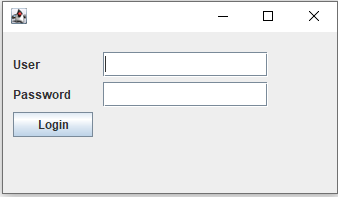
\includegraphics[width=.5\linewidth]{images/login.png}
	\caption{A bejelentkezés}
	\label{fig:login}
\end{figure}

\newpage
A bejelentkezésre kattintást kezelő kód a következő:

\begin{java}
@Override
public void actionPerformed(ActionEvent e) {
	
	String user = loginusertext.getText();
	@SuppressWarnings("deprecation")
	String password = loginpasswordtext.getText();
		
	if ((user.equals("test") || user.equals("admin"))
		&& (password.equals("admin") ||
	 	password.equals("test123"))) {
		LoginSuccessLabel.setText("Login successful");
		loginFrame.setVisible(false);
		Successgui.successgui();		
	} else if (user.equals("test") ||
	 	user.equals("admin")) {
		LoginSuccessLabel.setText
		("Login failed. Wrong password");
	} else if (password.equals("test123") ||
		 password.equals("admin")) {
		LoginSuccessLabel.setText
		("Login failed. Wrong User");
	} else
		LoginSuccessLabel.setText("Login failed");
		tries = tries + 1;
	if (tries == 3) {
		System.exit(0);
	}	
}	
\end{java}
\newpage
\section{A kezdőképernyő}	A bejelentkezés után a program kezdőképernyőjét \aref{fig:program}-es ábra mutatja. Ezen az ábrán lehet látni, hogy már egy lefuttatott parancs és annak az eredménye megjelent a konzolon. A program használata közben legtöbbször ezt a képernyőt látjuk.

\begin{figure} [H]
	\centering
	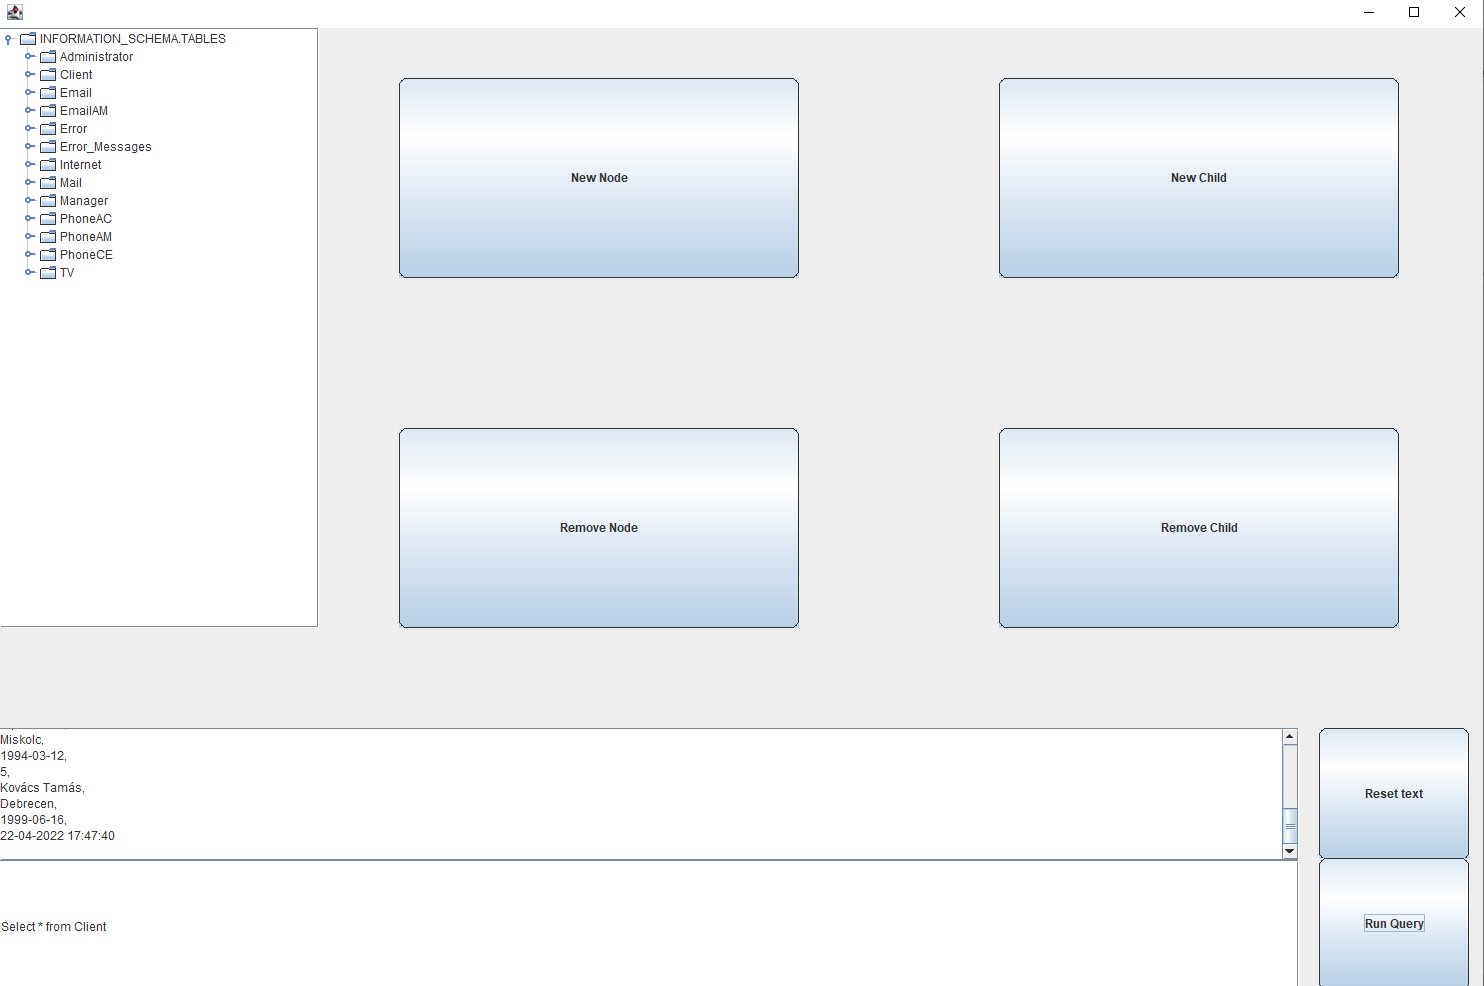
\includegraphics[width=.9\textwidth]{images/opening_screen.png}
	\caption{A kezdőképernyő}
	\label{fig:program}
\end{figure}

\section{Fa struktúra} A fa struktúra reprezentálja a csatolt adatbázis felépítését, annak minden táblájával. A tábláknak mappa ikonja van a táblákon belüli oszlopoknak pedig fájl ikonja. Az táblákat a struktúra csomópontként az oszlopokat pedig levélként kezeli, ezért a továbbiakban én is így fogok hivatkozni rájuk.\\

A fa struktúra alap állapotban \aref{fig:tree}-mas ábrán látható. Minden csomópontra és levélre rá tudunk kattintani a struktúrában, ami azt eredményezi, hogy a hozzárendelt adatokat kiírja a konzolon és hozzáadja a kiíratás dátumát. Miután egy csomópontra duplán kattintunk, az alatta lévő levelek megjelennek.

\begin{figure} [H]
	\centering
	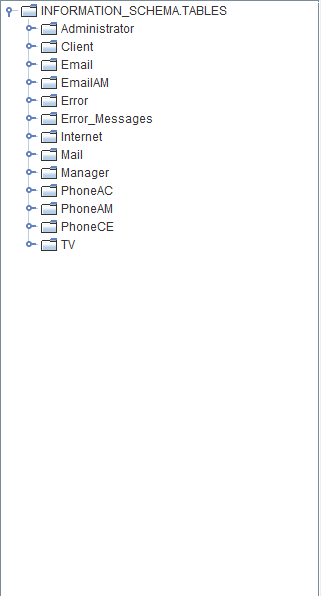
\includegraphics[height=.25\textheight]{images/tree.png}
	\caption{A fa struktúra}
	\label{fig:tree}
\end{figure}

Ha lenyitottuk az összes csomópontot, akkor a túl sok adat miatt, a struktúra jobb szélén egy legörgethető panel jelenik meg, amivel egyszerűen navigálhatunk a csomópontok és levelek között. Erre példát \aref{fig:treeexp}-es ábra mutat.

\begin{figure} [H]
	\centering
	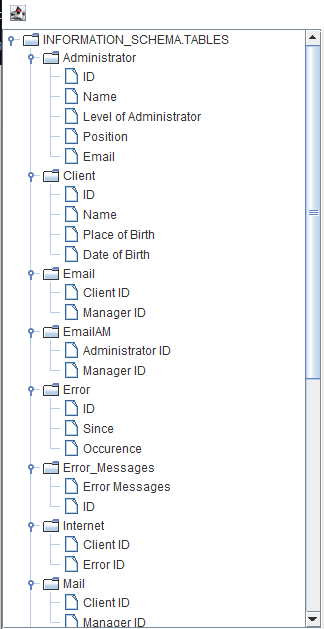
\includegraphics[height=.25\textheight]{images/tree_expanded.png}
	\caption{A fa struktúra lenyitva}
	\label{fig:treeexp}
\end{figure}

\section{Fa kezelő gombok} 4 gomb látható a kezdőképernyő felső részén, amik a fa struktúra módosítására készültek. Mind a négy gombnak különböző funkciója van ezekre külön-külön kitérek. Ezek a gombok láthatóak \aref{fig:program}-es ábrán és ránagyítva \aref{fig:modify} ábrán.

\begin{figure} [H]
	\centering
	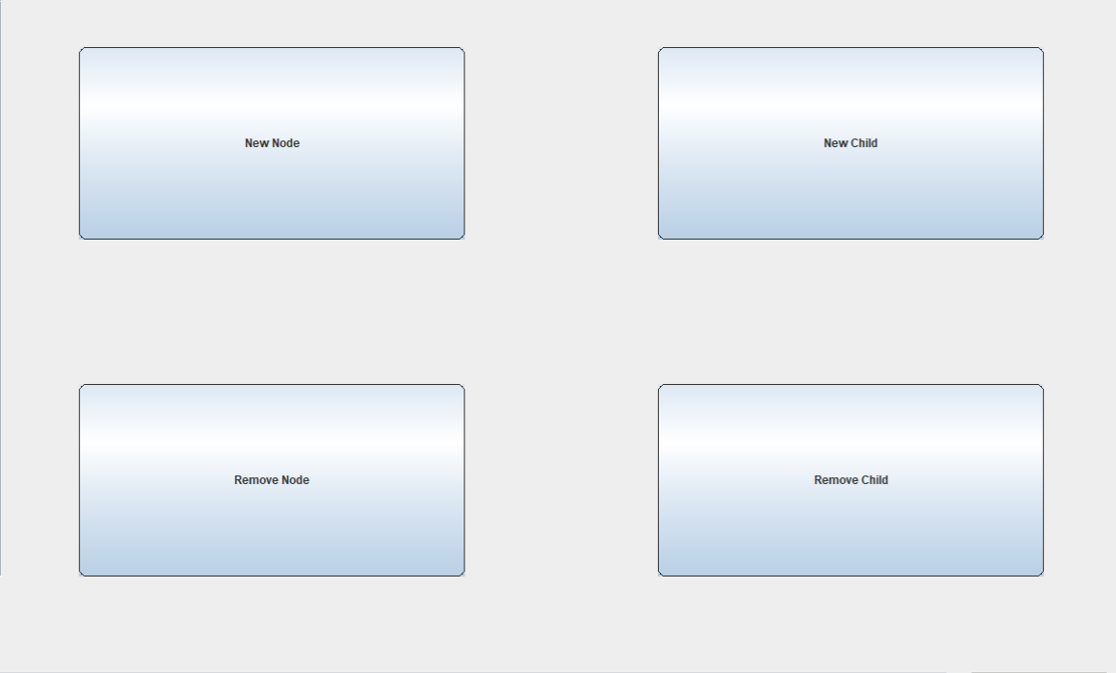
\includegraphics[height=.25\textheight]{images/node_buttons.png}
	\caption{A kezelő gombok}
	\label{fig:modify}
\end{figure}

Ha az új csomópont vagy az új levél gombra kattintunk, akkor eltűnik az alap 4 gomb és \aref{fig:modify_screen}-os ábrán látható gombok és sorok jelennek meg.

\begin{figure} [H]
	\centering
	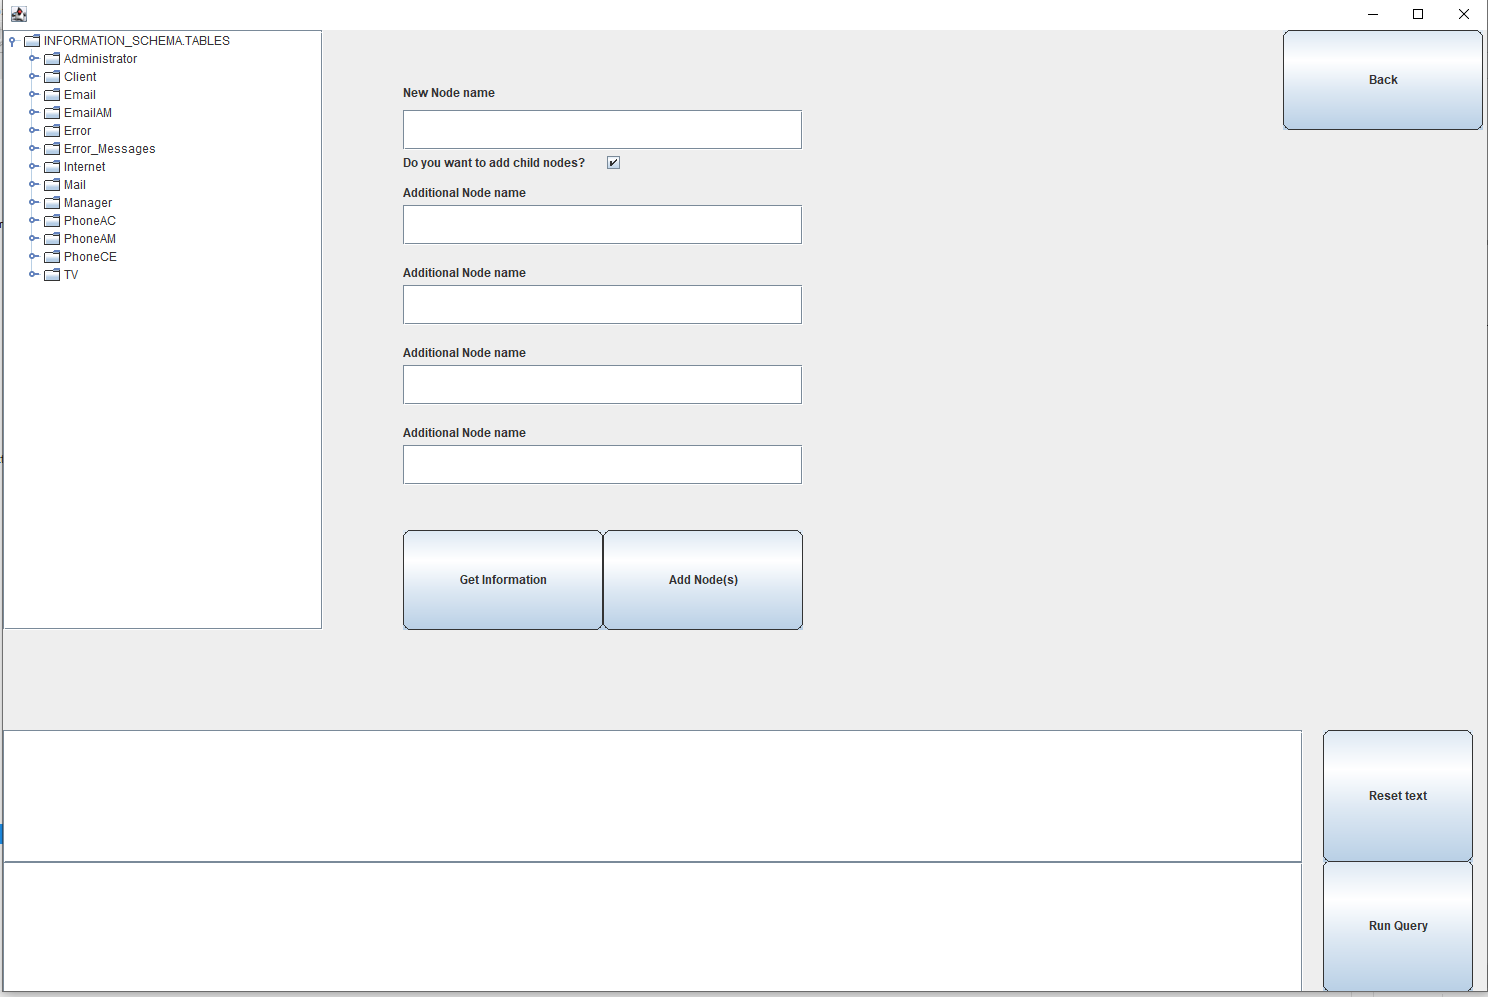
\includegraphics[width=.9\textwidth]{images/modify_screen.png}
	\caption{Az kezelő felület}
	\label{fig:modify_screen}
\end{figure}

\subsection{Új csomópont} Ezzel a gombbal lehetőségünk nyílik hozzáadni a fa struktúrához egy új csomópontot és ha szeretnénk alá több levelet is. A csomópont hozzáadásához először az információszerzés gombra kell kattintanunk, majd az új csomópont(ok) gombra.\\
Ha szeretnénk leveleket is hozzáadni, akkor először be kell pipálnunk a jelölőnégyzetet, amivel megjelenik a többi mező, ahova a beírt adatokat már levélként adjuk hozzá. Ehhez ugyanazt kell megtennünk, mintha új csomópontot raknánk hozzá, annyi különbséggel, hogy megjelenik egy új gomb az új csomópont(ok) mellett új levelekként és arra kell kattintanunk. 

\subsection{Új levél} A gomb működése hasonló az új csomópontéhoz. Először csak 1 mező lesz elérhető számunkra, viszont amint a jelölőnégyzetet bepipáljuk, megjelennek a további mezők. Ahhoz, hogy ez a funkció működjön, a fa struktúrában ki kell jelölni, hogy melyik csomóponthoz vagy levélhez szeretnénk további leveleket hozzáadni. Ha valamelyik mező üresen marad, akkor a program ezt jelzi nekünk a konzolon. Ahhoz, hogy a hozzáadás megtörténjen először az információszerzés gombra kell kattintani, majd az új levelek gombra.

\subsection{Csomópont törlés} A törlés gombok máshogy működnek mint a hozzáadás gombok. Ha elemet szeretnénk törölni, akkor figyelni kell rá, hogy ez az összes hozzá tartozó levelet is törölni fogja kérdezés nélkül. A törlés menete egyszerű. Ki kell jelölni a fán, hogy melyik csomópontot szeretnénk törölni, majd rá kattintani a csomópont törlése gombot.

\subsection{Levél törlés} A levél törlés gomb hasonlóan működik, mint a csomópont törlés. A különbség a kettő között, hogy ezzel csak és kimondottan leveleket lehet törölni. Ha egy csomópontot próbálnánk vele törölni, akkor a konzolon megjelenik a hozzá tartozó hibaüzenet. A törlés menete ugyanaz, mint a csomópontnál. Először kijelölésre kerül a levél, majd a gombra kattintás után az eltűnik a fából.

\section{Konzol} A konzol tartalmaz 2 beviteli mezőt és 2 gombot. A felső beviteli mező csak arra szolgál, hogy a kiadott parancsok eredményét, illetve a hibaüzeneteket kiírja egy időponttal ellátva. A két gomb az alsó beviteli mezővel foglalkozik. A szöveg alaphelyzetbe állítás gombbal az alsó mezőben lévő szöveget ki lehet törölni és vissza állítani alap helyzetbe, amíg a parancs futtatás gombbal ebbe a mezőbe beírt SQL parancsot lehet lefuttatni.


